\section{给定释放条件下的泥石流传播与模型比较}\label{q4-section}

\subsection{空间构型与释放设计}

本节将前述稳定性计算中的物源状态转为流动初始条件，研究流深、速度、展布与下游响应。共完成24项一维沿程、10项自编二维计算，以及31项原生求解：单混合物18项、复合固水3项、D-Claw孔压9项，另有1项通用材料诊断。原生队列包含30项目标材料计算；7项材料映射不适用的配置另列。由此形成简化动力学、均质混合物、孔压耦合和相间运动四个层次的过程比较。

地形采用Copernicus GLO-30，统一至UTM 45N及60、120 m格网；产品垂直基准为EGM2008，主体获取于2011—2015年\cite{q4-dem}。在候选源面与河谷构型上得到20.70、21.42、21.66 km三条地形路径，源边缘接河的局部连接长约0.710—0.939 km。该构型为源面、河道与代表目标提供一致的计算坐标；地形年代和图上对象定位作为几何条件保留。

表\ref{q4-tab-design}将4个机械设计映射为7个传播运行。紧凑源按Q2给出的面积、厚度与体积投影；全源面使用共同候选掩膜。60 m源格面积为0.9252 km$^2$，120 m为0.9648 km$^2$，后者按相同体积归一厚度。主过程选取全源面p0036--ST／120 m：体积$31.184139\times10^6$ m$^3$，初始垂直厚度32.322 m，等效密度2158.626 kg/m$^3$。各释放初速为零。H描述结构内的储排水作用，SH、STH的释放自由水体积分数仍为0；在这组单混合物运行中，岩冰组分通过体积和等效密度进入传播。

\begin{table}[htbp]
\centering\small
\caption{四个机械设计的释放映射；体积单位为$10^6$ m$^3$}\label{q4-tab-design}
\begin{tabularx}{\linewidth}{lrrrrY}
\toprule
设计 & 密度(kg/m$^3$) & 紧凑源体积 & 全源面体积 & 运行数 & 格网(m)\\
\midrule
p0000--S &1298.435&0.559400&51.755729&2&60；60\\
p0036--ST&2158.626&1.348212&31.184139&3&60；60、120\\
p0072--SH&1293.058&5.100007&---&1&60\\
p0255--STH&1708.464&1.255515&---&1&60\\
\bottomrule
\end{tabularx}
\par\raggedright\footnotesize 格网列依次对应紧凑源与全源面；破折号表示该映射未纳入此组运行。7次运行共享4个机械设计，形成49条目标记录，不赋予统计权重。S、SH保留“若整体释放”的条件。
\end{table}

\subsection{深度平均动力学与响应定义}

采用r.avaflow 4.0 Rev7组织单混合物及相模型计算\cite{q4-ravaflow,q4-multiphase}，自编有限体积模型提供一维、二维对照。其共同质量形式为
\begin{equation}
\frac{\partial h}{\partial\tau}+\nabla\!\cdot(h\boldsymbol u)=E,
\qquad \tau=t-t_{\mathrm{release}},
\label{q4-eq-mass}
\end{equation}
自编对照采用有限体积形式交换厚度和动量：二维计算保留两个水平分量，一维则沿三条路线转换距离—高程，并用恒定等效宽度组织质量账。相模型对各相保存$(h_k,h_ku_k,h_kv_k)$，相加得到总厚度；因此，一维的等效宽度面积、二维平面足迹及分相状态分别解释。

其中$h$为流深，$\boldsymbol u$为水平速度，$E$为单位面积夹带源项；$t$沿用全文UTC时间，$\tau$为给定整体释放后的秒数。动量过程可归纳为通量、重力、阻力、相间作用及物源交换：
\begin{equation}
\begin{aligned}
\frac{\partial\boldsymbol q}{\partial\tau}+\nabla\!\cdot\boldsymbol F(\boldsymbol q)
&=\boldsymbol S_g+\boldsymbol S_f+\boldsymbol S_{\mathrm{inter}}+\boldsymbol S_E,\\
\frac{\boldsymbol\tau_b}{\rho}
&=\left(\mu g_nh+\frac{g\lVert\boldsymbol u\rVert^2}{\xi}\right)
\frac{\boldsymbol u}{\lVert\boldsymbol u\rVert+\varepsilon}.
\end{aligned}
\label{q4-eq-momentum}
\end{equation}
$\boldsymbol q$为厚度与水平动量组成的状态向量。第二行给出单混合物对照的Coulomb--Voellmy阻力表达；主设置$\mu=0.15$、$\xi=1000$ m/s$^2$，小量$\varepsilon$仅用于零速方向正则化。原生求解器保留自身地形、压力和数值闭合，跨模型比较以各自实际状态量为准。请求时域统一为1800 s，名义输出间隔20 s，时间步由CFL控制；实际存帧时刻直接读取原生记录，避免以固定间隔替代真实积分时间。

孔压路线采用D-Claw 1.0\cite{q4-dclaw,q4-dclaw-code}，以固相体积分数、剪胀及基底孔压$p_b$耦合流动，有效抗力由$(\rho g_nh-p_b)\tan\phi$控制。本组孔压参考的初始固相体积分数为0.63，参考渗透率取$10^{-10}$ m$^2$；它们是所采用算例设置的迁移参数。复合相路线将岩0.6、冰0.1合为体积分数0.7的固体，其密度为2445.286 kg/m$^3$，水相占0.3；中间固相为空。它描述复合固体与水的相对运动，冰的作用限于密度闭合，相变与岩冰相对速度不在该配置中求解。孔压及复合相参考释放体积均为13.878$\times10^6$ m$^3$，与主ST物源分别定义。

所有目标使用代表点周围100 m内的格心，总厚度阈值统一为0.1 m。令$\mathcal B_j$为该邻域，首个存帧响应为
\begin{equation}
\widehat\tau_j=\min\{\tau_k:\max_{\boldsymbol x_i\in\mathcal B_j}h_i(\tau_k)\geq0.1\},
\qquad \tau_j\in(\tau_{k-1},\tau_k].
\label{q4-eq-arrival}
\end{equation}
图中J、P分别为汇流与口岸代表点；另5个OSM几何对应3个实体。累计足迹按请求1800 s内的保存帧最大厚度统计，速度为湿区水平模长（相模型取湿相最大值），区别于原生逐步累计的地形标量速度。机械启动至整体释放的延迟保持未知，结果据此解释为相对释放响应。

\subsection{沿谷传播过程与模型状态}

\begin{figure}[H]
\centering
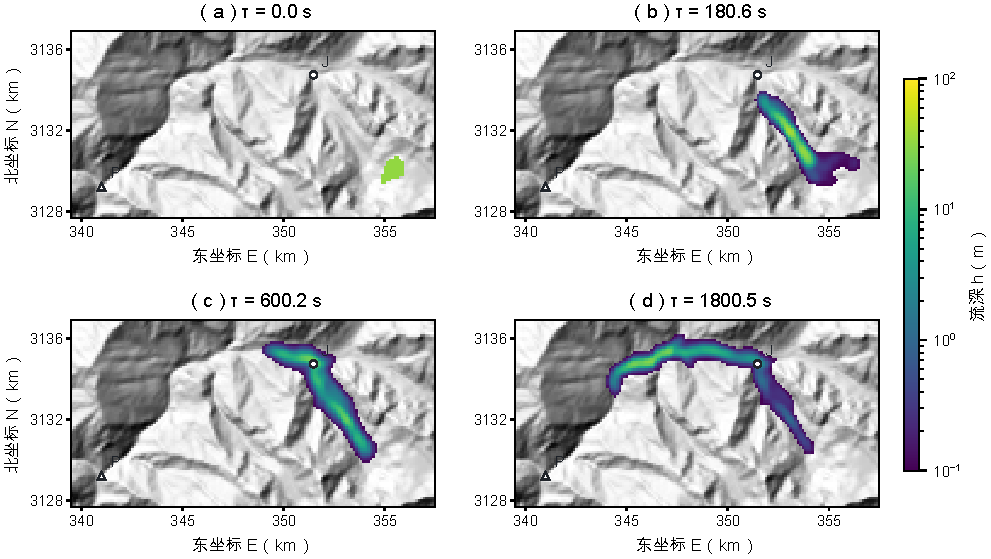
\includegraphics[width=\linewidth]{figures/q4/process_fullmask_st120.pdf}
\caption{全源面ST／120 m的流深过程。灰底为地形阴影，色标为对数流深，J、P为目标代表点；时刻取原生实际存帧，末帧1800.5 s单列展示。}\label{q4-fig-process}
\end{figure}

图\ref{q4-fig-process}展示主ST运行由源区展布、进入主沟到汇流后沿谷运动的过程。0、180.6、600.2、1800.5 s的当时湿区面积依次为0.9648、7.2576、10.4400、13.3056 km$^2$。180.6 s时流体仍主要分布在源区下方沟段；600.2 s已越过汇流代表点并向西展布，末态沿谷形成连续流动带。四帧局部最大流深为32.322、40.337、22.739、28.366 m，说明局部增厚与整体扩散同时发生；当时湿区面积与全程累计足迹承担不同的过程描述。



主ST运行的保存帧峰深为61.616 m，湿区水平峰速74.066 m/s，汇流响应位于释放后(240.6,260.1] s。保持体积、密度与阻力，将格网改为60 m，峰深增至80.906 m、水平峰速降至67.437 m/s，累计足迹由23.0112降至12.1608 km$^2$；两个汇流括号有0.1 s交叠。图\ref{q4-fig-comparison}上排显示，加密格网使主要运动带更窄，局部厚度更集中。因此，局部极值、平面足迹和前缘响应共同刻画传播强度及其尺度变化。

\begin{table}[htbp]
\centering\small
\caption{代表运行的保存帧过程指标}\label{q4-tab-response}
\begin{tabularx}{\linewidth}{lrrrrY}
\toprule
运行 & 体积($10^6$m$^3$)&峰深(m)&峰速(m/s)&足迹(km$^2$)&汇流括号(s)\\
\midrule
ST全源面／120 m&31.184&61.616&74.066&23.0112&(240.6,260.1]\\
ST全源面／60 m &31.184&80.906&67.437&12.1608&(221.0,240.7]\\
D-Claw扩域／120 m&13.878&60.899&180.494&83.3904&(40,60]\\
复合固水／120 m&13.878&22.005&66.082&29.3904&(200.0,220.4]\\
\bottomrule
\end{tabularx}
\par\raggedright\footnotesize 足迹为1800 s内保存帧总厚最大值达到0.1 m的平面面积，峰速采用湿区水平速度；D-Claw为整个扩展域，图中仅显示共同核心区域。不同物源、初始化和相闭合分别保持，表内数值用于结构对照。
\end{table}

D-Claw增加了压力与固相状态的空间解释：扩域运行的汇流响应为(40,60] s，口岸代表点为(160,180] s；图\ref{q4-fig-comparison}下排给出180 s的基底压力场。复合固水运行则输出各相厚度及水相份额，汇流响应为(200.0,220.4] s。主ST的口岸代表点在本时域内没有厚度达阈记录。这些响应共同反映了给定物源和闭合结构的差异；其中D-Claw初态积分使源厚支持由67格扩为111格，厚度归一$L_1$差13.899\%，跨框架速度差因而同时包含初态映射与动力过程的作用。

\begin{figure}[H]
\centering
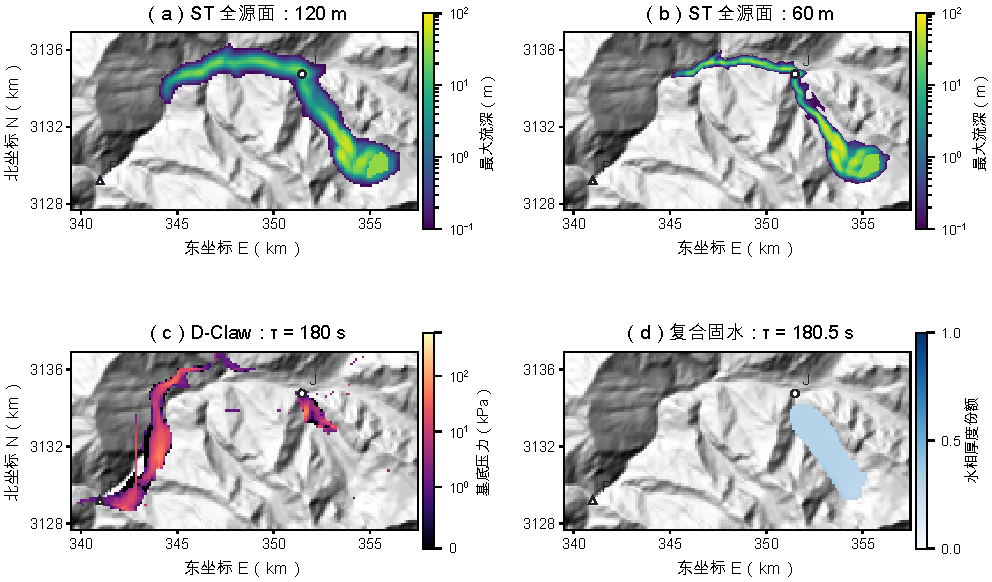
\includegraphics[width=\linewidth]{figures/q4/model_comparison.pdf}
\caption{格网与物理结构对照。上排为ST双格网1800 s内累计最大流深；下排分别为扩域D-Claw的180 s基底压力和复合固水的180.5 s水相厚度份额。压力色阶在1 kPa以上采用对数间隔；下排使用各自13.878$\times10^6$ m$^3$参考释放。}\label{q4-fig-comparison}
\end{figure}

七个跨问运行中，全源面S的汇流响应为(161.1,180.2] s；紧凑源ST、SH、STH分别为(1360.5,1380.1]、(801.1,820.6]、(1400.1,1420.5] s，紧凑源S在时域内无达阈记录。几何和物源规模改变了运动带及响应时标，因而49条记录按父设计、源面与格网关联保存，不将不同物源的时延直接合并成概率分布。

\subsection{源项、数值响应与过程解释}

表\ref{q4-tab-numerics}集中比较数值和物理干预。15~m释放厚度的120~m格网参考只将CFL从0.5减至0.25，水平保存峰速即由92.394降至53.256 m/s，原生累计地形标量也由152.356降至92.633 m/s。两类速度均呈响应，时间步效应包含存帧采样之外的数值变化。60 m参考的质量账为+11.506\%，与120 m的$-1.026\%$相对照，说明格网、初态映射和源面陡坎共同影响预算。自编模型提供另一组证据：含边界项的体积账最大相对残差为$8.05\times10^{-16}$，而常坡薄流20、10、5 m格网速度相对误差依次为0.755、0.377、0.188；守恒与传播速度应作为互补评价量。

\begin{table}[htbp]
\centering\small
\caption{参考物源的源项、格网与耦合对照}\label{q4-tab-numerics}
\begin{tabularx}{\linewidth}{lrrY}
\toprule
运行／干预 & 水平峰速(m/s)&末态质量账(\%)&过程响应\\
\midrule
单相120 m，CFL=0.5 &92.394&$-1.026$&汇流(420.9,441.3] s\\
单相120 m，CFL=0.25&53.256&$-1.551$&汇流(461.0,480.7] s\\
单相60 m，CFL=0.5&59.596&$+11.506$&汇流(540.1,560.8] s\\
复合固水，保留耦合&66.082&$-10.301$&汇流(200.0,220.4] s\\
复合固水，关闭drag／VM&---&$-1.984$&汇流(181.1,200.4] s\\
全岩固体＋水&---&$-13.145$&汇流(220.1,240.2] s\\
D-Claw扩域&180.494&$-4.147$&口岸(160,180] s\\
单相120 m，1 m侵蚀床&---&$-1.157$&夹带5.61843$\times10^6$ m$^3$\\
\bottomrule
\end{tabularx}
\par\raggedright\footnotesize 单相参考$V=13.878\times10^6$ m$^3$、$\rho=2105$ kg/m$^3$；相模型及孔压模型采用各自组分密度。r.avaflow列原生终态预算，单列边缘储库及侵蚀源；D-Claw列扩域总质量变化。实际末时为1800—1802.4 s。横线表示本表不重复列该量。
\end{table}

物理干预提供了可分解的过程量。复合固水与全岩配对保持初始相厚及总体积，固相密度改变使总质量随之变化；关闭的仅为drag与virtual-mass两项，压力和浮力等项继续保留。全岩与复合参考的汇流括号交叠0.3~s，关闭drag／VM与复合参考交叠0.4~s，应结合响应和质量账解释。D-Claw扩大域后所有保存外缘的厚度与水平动量均为零，口岸括号保持不变，同时总质量在180 s和1800 s分别变化$-2.161\%$、$-4.147\%$，为边界敏感性与域内预算提供了独立信息。

有界夹带将路径缓冲区内1 m床层作为物源，容量9.5472$\times10^6$ m$^3$，实际加入5.61843$\times10^6$ m$^3$。扣除该新增源后再讨论预算，可区分侵蚀增长与数值残差。末态以$h\geq0.1$ m、湿相（厚度下限$10^{-6}$ m）最大水平速度小于0.1 m/s定义静止残余：参考及夹带两例此集合为空，$\mu=0.25$运行则得到约0.3805$\times10^6$ m$^3$有限时刻残余。因此，累计最大流深、末态流深与静止残余分别对应最大过流厚度、当时展布与停滞状态，永久堆积需要更长时段及沉积观测解释。

本节以全源面ST过程串联物源、沿谷展布与代表目标响应，双格网、孔压、复合相及有界夹带分别增加空间分辨率、有效应力、组分和源项的信息。本文以相对释放时钟、给定参数与源面组织情景，形成可复查的传播过程、目标响应和结构敏感性结果；与源区机械状态的联系按同一情景标识保留阶段转换项。

\AIcredit
\FloatBarrier
